
%(BEGIN_QUESTION)
% Copyright 2011, Tony R. Kuphaldt, released under the Creative Commons Attribution License (v 1.0)
% This means you may do almost anything with this work of mine, so long as you give me proper credit

Bestem regulatorens virkningsretning ({\it direct} eller {\it reverse}) ved å analysere programkoden:

$$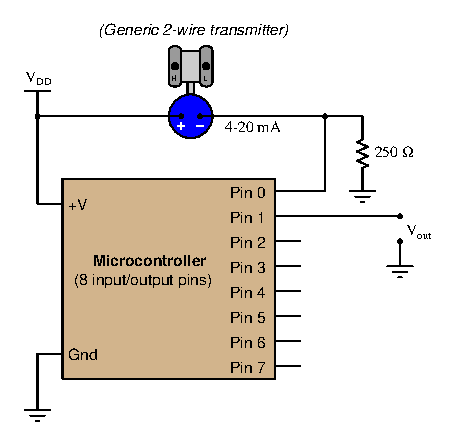
\includegraphics[width=15.5cm]{i00896x01.eps}$$

\hbox{ \vrule
\vbox{ \hrule \vskip 3pt
\hbox{ \hskip 3pt
\vbox{ \hsize=5in \raggedright

\noindent
\underbar{\bf Pseudokodeliste}

{\tt Declare Pin0 as an analog input (scale 0 to 5 volts = 0 to 1023)}

{\tt Declare Pin1 as an analog output (scale 0 to 5 volts = 0 to 1023)}

{\tt Declare SP as a variable, initially set to a value of 614}

{\tt Declare GAIN as a variable, initially set to a value of 1.0}

{\tt Declare ERROR as a variable}

{\tt Declare BIAS as a variable, initially set to a value of 614}

\vskip 10pt

{\tt LOOP}

\hskip 10pt {\tt SET ERROR = SP - Pin0}

\hskip 10pt {\tt SET Pin1 = (GAIN * ERROR) + BIAS}

{\tt ENDLOOP}
}
\hskip 3pt}%
\vskip 5pt \hrule}%
\vrule}

\vskip 10pt

Anta nå at du ikke kan endre programkoden, men kun verdiene til variablene {\tt GAIN} og {\tt BIAS}, samt elektriske tilkoblinger til regulatoren. Finn en måte å bytte regulatorvirkningen til motsatt retning.

\underbar{file i00896}
%(END_QUESTION)





%(BEGIN_ANSWER)

Jeg anbefaler 5 poeng for riktig virkning og 5 poeng for en fungerende løsning:

\vskip 10pt

Virkningen slik den er programmert er {\bf reverse}. For å få direct virkning kan du sette {\tt GAIN} til en negativ verdi i stedet for positiv.

%(END_ANSWER)





%(BEGIN_NOTES)

{\bf Denne oppgaven er ment kun for eksamen, ikke for arbeidsark!}.

%(END_NOTES)
